% Software Roboter (C++)
% Zuständig: Leander

\section{Software - Roboter}
\label{sec:software_robots}
Für die Programmierung der Mikrocontroller verwenden wir PlatformIO.
%
PlatformIO ist eine Alternative zur Arduino-IDE,
welche mithilfe von Plugins in viele IDEs wie z.B. VSCode und CLion integriert werden kann.
%
Alternativ kann man PlatformIO auch über die Kommandozeile bedienen.
%
Vorteile von PlatformIO gegenüber der Arduino-IDE sind u.A. schnelleres Kompilieren,
ordentliche Auto-Vervollständigung,
statische Code-Analyse (Linting),
und ein schön geregeltes System für Bibliotheken.

\subsection{Kameras}
\label{subsec:robots_cams}
Wir verwenden jeweils ein ESP32-CAM AI-Thinker Modul zur erweiterten
Fernüberwachung der Roboter.
%
Dieses verbindet sich über WLAN mit dem \texttt{IoT}-Netzwerk und bietet über HTTP einen MJPEG-Videostream an.
%
Die drei Videostreams (einer pro Roboter) werden dann im Web-Interface
zusätzlich zu den LiDAR-Umgebungsdaten angezeigt,
um das räumliche Vorstellungsvermögen der Benutzer zu unterstützen.
\begin{figure}[H]
    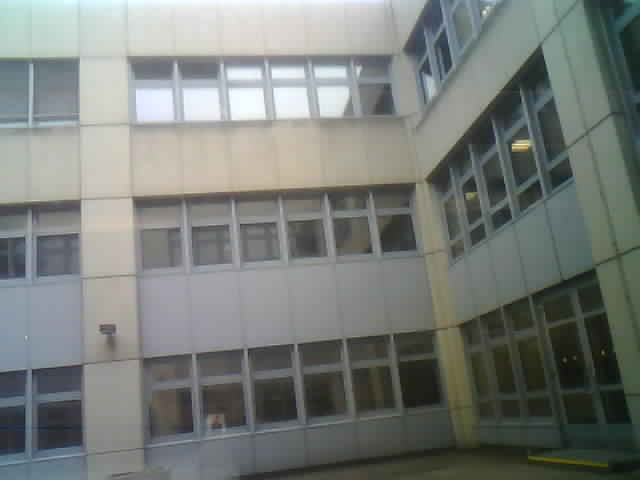
\includegraphics[width=0.7\textwidth, center]{img/cam_erstes_bild.png}
    \caption{Erstes empfangenes Bild der ESP32-CAM}
    \label{fig:cam_erstes_bild}
\end{figure}

\subsection{Core-Bibliothek}
\label{subec:robots_core}

\subsection{Guide}
\label{subsec:software_guide}

\subsection{Tamerlan}
\label{subsec:software_tamerlan}

\subsection{Bambi}
\label{subsec:software_bambi}